\documentclass[a4paper,12pt,stu,donotrepeattitle,floatsintext,twoside]{apa7}

\usepackage{MAE}

\begin{document}

\begin{titlepage}
    \thispagestyle{empty} % Cover page must have no page number.
    \centering % Center everything on the cover page.

    \vspace{5\baselineskip}

    \fontfamily{phv}\fontencoding{T1}
    \fontsize{24}{20pt}\fontseries{b}\selectfont
    \titlet\par
    \vspace{2.5\baselineskip}

    % Print author's name
    \fontsize{16}{12pt}\fontseries{m}\fontshape{n}\selectfont \authort\par
    \vspace{2.5\baselineskip}
    \hrulefill
    \vspace{2.5\baselineskip}
    
\includegraphics[width=\linewidth]{01_uio_full_logo_eng_pos.eps}\\[\baselineskip]

    % Print degree name
    \fontsize{16}{16pt}\fontseries{m}\fontshape{n}\selectfont Master of Science in Assessment, Measurement and Evaluation\\
    \fontsize{16}{16pt}\fontseries{m}\fontshape{n}\selectfont 30 credits master thesis\\[1.5\baselineskip]

    % Print CEMO's name
    \fontsize{16}{12pt}\fontseries{m}\fontshape{n}\selectfont CEMO: Centre for Educational Measurement\\
    \fontsize{16}{12pt}\fontseries{m}\fontshape{n}\selectfont Faculty of Educational Sciences\\[1.5\baselineskip]
    \fontsize{12}{12pt}\fontseries{m}\fontshape{n}\selectfont \semester\par
\end{titlepage}
\cleardoublepage

%%%%%%%%%%%%%%%%%%%%%%%%%%%%%%%%%%%%%%%%%%%%%%%%%%%%%%%%%%%%%%%%%%%%%%%%%%%%%%%%
%%%%%%%%%%%%%%%%%%%%%%%%% ABSTRACTS & ACKNOWLEDGEMENTS %%%%%%%%%%%%%%%%%%%%%%%%%
%%%%%%%%%%%%%%%%%%%%%%%%%%%%%%%%%%%%%%%%%%%%%%%%%%%%%%%%%%%%%%%%%%%%%%%%%%%%%%%%

% Switch page numbering to roman for preambles
\pagenumbering{roman}

\section*{Popular Abstract}

\noindent Maximum half a page. One single paragraph. No indentation. Nunc sed risus diam. Nam vel neque mi. Fusce pretium a erat nec placerat. Proin faucibus finibus aliquet. Phasellus ut felis feugiat, tempus enim eget, ornare neque. Ut magna ante, faucibus eget pellentesque dictum, dapibus sed libero. Integer hendrerit lacus id lacus sodales vehicula. Curabitur orci tortor, condimentum quis velit in, tincidunt convallis turpis. Sed eget auctor est, et aliquet ipsum. Pellentesque habitant morbi tristique senectus et netus et malesuada fames ac turpis egestas. Etiam vel risus eget velit consectetur blandit. Fusce vitae nulla sapien. Vestibulum luctus neque quis risus laoreet, ac faucibus turpis tristique. Nunc a nunc eget odio fringilla tempus.

\newpage

\section*{Acknowledgements}

Maecenas vel maximus erat. Vestibulum ac ornare neque. Integer vestibulum elit sem, ac varius turpis dapibus sed. Nulla erat neque, consectetur nec urna pretium, finibus elementum urna. Donec id hendrerit sem. Cras et arcu nunc. Nam dictum lacus vitae lorem luctus ultricies. Suspendisse varius velit quis imperdiet rhoncus. Quisque ut placerat nulla. Cras ut tortor mattis, finibus nisi non, sollicitudin purus. Vestibulum dolor elit, accumsan id ligula eget, lobortis malesuada lorem. Aenean vel maximus justo.

Proin pretium venenatis tortor, id varius turpis semper non. Sed non elit eget purus cursus ultrices et sit amet diam. Morbi vestibulum tortor magna, sed placerat justo condimentum ac. Morbi leo magna, pharetra in neque eget, fringilla aliquam elit. Duis at ultrices ligula. Suspendisse ac ligula in tortor condimentum feugiat. Etiam ut ligula id sapien efficitur malesuada. Sed nec sagittis nisi, nec auctor dolor. Proin viverra feugiat gravida. Quisque venenatis a risus non venenatis.

% Insert a blank page if preamble ends on an odd page so Page 1 starts right.
\cleardoublepage

%%%%%%%%%%%%%%%%%%%%%%%%%%%%%%%%%%%%%%%%%%%%%%%%%%%%%%%%%%%%%%%%%%%%%%%%%%%%%%%%
%%%%%%%%%%%%%%%%%%%%%%%% CORE OF MANUSCRIPT STARTS HERE %%%%%%%%%%%%%%%%%%%%%%%%
%%%%%%%%%%%%%%%%%%%%%%%%%%%%%%%%%%%%%%%%%%%%%%%%%%%%%%%%%%%%%%%%%%%%%%%%%%%%%%%%

% Arabic page numbers for main text
\pagenumbering{arabic}

\section{\titlet}
\vspace{0.5\baselineskip}   % Insert a line between title and abstract

{% Indent both left and right margins of abstract by 0.5 in.
\leftskip0.5in\relax
\rightskip0.5in\relax
% APA7 Rule 2.9 Abstract
% Abstracts in paragraph format are written as a single paragraph without indentation of the first line.
% APA7 Rule 2.24 Paragraph indentation
% Exception dot point 4: The first line of the abstract should be flush left.
\noindent Single paragraph. No indentation. Maximum 250 words. Phasellus egestas purus et sem porta venenatis. Vestibulum ante ipsum primis in faucibus orci luctus et ultrices posuere cubilia curae; Sed pulvinar leo ut posuere sollicitudin. Integer sem tortor, tristique id nisl sed, aliquam pharetra tortor. Integer tortor purus, facilisis mollis tortor nec, sodales bibendum urna. Nulla quam enim, feugiat semper neque ut, sagittis ullamcorper urna. Donec et iaculis mi. Etiam congue tellus ut felis viverra, ac mollis eros venenatis. Vivamus eget ante at eros pulvinar tempor nec at arcu. Donec et vestibulum nunc. Fusce sed metus nisi. In leo turpis, mattis a tincidunt luctus, pellentesque et velit. Ut tortor mi, rutrum nec fringilla vitae, maximus et ligula. Vestibulum finibus semper ornare.

% APA7 Rule 2.10 Keywords
% Write the label "Keywords:" (in italic) one line below the abstract, indented 0.5 in. like a regular paragraph, followed by the keywords in lowercase (but capitalize proper nouns), separated by commas. The key words can be listed in any order. Do not use a period or other punctuation after the last keyword. If the keywords run onto a second line, the second line is not indented.
\textit{Keywords:} keyword 1, keyword 2, keyword 3
% Leave an empty line behind
\vspace{0.75\baselineskip}
}

% Never start the introduction with a heading "Introduction". Simply start your first paragraph.

Maecenas nec ultricies tellus. Suspendisse tristique a ante non fringilla. Morbi et sem dignissim, aliquet leo vel, scelerisque purus. Sed iaculis, est vel molestie consequat, erat elit venenatis arcu, a tempor libero diam sit amet velit. Donec ut vestibulum lectus, ut fermentum turpis. Etiam rutrum eros a sem commodo consequat \parencite{Ludtkeetal2008}.

\subsection{Level 2 Heading}

Suspendisse varius iaculis sem, vel congue augue vulputate in. Vestibulum ante ipsum primis in faucibus orci luctus et ultrices posuere cubilia curae; Nullam vitae purus eget purus eleifend gravida finibus eget erat. Quisque eget tincidunt dolor. In ac lectus at lectus cursus scelerisque non a libero.

Donec posuere neque vitae sapien aliquet maximus. Phasellus malesuada, lectus eget molestie facilisis, mauris nunc congue risus, in hendrerit magna dolor sit amet eros. Phasellus nec elit nibh. Praesent eget leo id enim blandit elementum \parencite{Marshetal2009}.

\subsubsection{Level 3 Heading}

\textcite{Marshetal2009} nulla finibus dignissim ex vitae mattis. Phasellus ligula sapien, auctor vel finibus non, fermentum a diam. Ut commodo leo porttitor libero porta, ac accumsan ante egestas. Vivamus in sem eu felis interdum vulputate. Vivamus ut orci libero.

Fusce et faucibus dolor. Aliquam erat volutpat. Quisque sagittis justo vitae dui posuere, a aliquet nunc ornare. Praesent tempor a est ac mattis. Interdum et malesuada fames ac ante ipsum primis in faucibus. Proin elementum luctus placerat. Sed rhoncus leo in magna cursus egestas.

\paragraph{Level 4 Heading}

Fusce at sem in est varius consequat. Donec magna arcu, placerat non rhoncus id, ultricies at tortor. Curabitur id sem ac lectus pretium dignissim. Etiam faucibus, dolor ac egestas efficitur, dolor arcu posuere tellus, eget elementum est velit eget risus. Suspendisse potenti.

\paragraph{Level 4 Heading}

Praesent eu ornare ipsum. Sed mauris tortor, pretium dignissim pellentesque et, pulvinar in augue. Nunc maximus risus diam, in rhoncus augue placerat vitae. Etiam libero quam, mattis ut nulla sed, pellentesque iaculis neque. Vestibulum consectetur ex ipsum, quis fermentum mauris venenatis sit amet.

\subsubsection{Level 3 Heading}

Nullam id commodo turpis. Pellentesque sed fermentum quam. Aenean ut massa id quam pretium blandit ac in ex. Morbi ultricies tellus magna. Quisque ornare, ligula at tincidunt finibus, justo mauris tristique lectus, at bibendum odio sapien sed ante. Curabitur ultrices pulvinar magna quis feugiat.


\section{Method}\label{sec:Method}

Aenean egestas, magna vitae venenatis tincidunt, lacus nunc suscipit mauris, eu tincidunt enim nulla et leo. Ut tincidunt ante at mauris semper hendrerit. Nam consectetur aliquet est sit amet accumsan. Pellentesque porta nisl sapien. Ut vel vulputate est.

\subsection{Sample}

Mauris eu efficitur lectus, id suscipit enim. Phasellus justo nunc, gravida sed pulvinar nec, hendrerit quis orci. Nulla quis interdum augue. Vestibulum augue orci, porta nec erat vitae, bibendum ullamcorper massa.

\subsection{Measures}

Suspendisse potenti. Quisque nec interdum nunc. Curabitur tempus nibh non magna porttitor sodales. Donec nec lacus nibh. Phasellus pretium vehicula pretium. In vitae libero tempor, ullamcorper massa nec, ultrices nunc.

\subsection{Statistical Analysis}

Phasellus eget lorem vitae ligula ultrices scelerisque. Curabitur lacinia, magna in interdum faucibus, nibh magna vestibulum risus, eget ornare justo ante in ex. Vivamus ullamcorper commodo erat, a iaculis tortor congue scelerisque.

\begin{equation}\label{eq:mcsquare}
    E=mc^2
\end{equation}

Curabitur viverra velit lacus, sed hendrerit augue dictum egestas. Suspendisse ipsum sem, molestie tempus nulla vitae, faucibus rhoncus massa. Maecenas tempus, eros vel tempus laoreet, risus tortor ultrices diam, a blandit nisl velit non purus. Etiam id rutrum mi (see \cref{eq:mcsquare}).

\section{Results}
\label{sec:4}

Donec vitae efficitur sapien. Sed nisl ante, rutrum ac risus nec, mattis facilisis mauris. Quisque eu faucibus nisi, at viverra tortor. Proin semper velit eu mauris vestibulum faucibus. Sed venenatis risus id est pretium pretium (see \cref{tab:simple}).

Nulla condimentum nec velit sed mattis. Duis congue ut erat eget malesuada. Proin eget lorem sodales, varius dolor ut, vestibulum arcu. Praesent risus enim, hendrerit ut malesuada ut, vulputate posuere lectus.

\MAEtable{tab:simple}{Simple Table}{
    \begin{tabular}{ccc}
        \hline
        Head1 & Head2 & Head3 \\
        \hline
        cell1 & cell2 & cell3 \\
        cell4 & cell5 & cell6 \\
        cell7 & cell8 & cell9 \\
        \hline
    \end{tabular}
}{This is a very simple table.}{}

\subsection{A Generic Level 2 Heading}

Suspendisse laoreet, tortor nec interdum malesuada, risus tortor malesuada leo, sit amet blandit ligula turpis vitae lectus. Nullam pulvinar sollicitudin arcu ut sagittis. Vestibulum mattis justo vel nibh ultricies dictum. Ut rhoncus tortor vitae quam viverra congue. Morbi lobortis tortor et lacinia vestibulum (see~\cref{fig:hist}).

% \MAEfig{fig:example}{Example Figure}{File}{Noteblabla}{p}
\MAEfig{fig:hist}{Histogram of 100 Random Numbers}{hist.eps}{This histogram shows the frequency distribution of 100 random numbers drawn from the standard normal distribution $N(0,1)$ using seed 2020.}{}

Aenean cursus fringilla maximus. Lorem ipsum dolor sit amet, consectetur adipiscing elit. Integer semper est velit, nec hendrerit nisl convallis ut. Donec ornare leo quis egestas elementum.

\subsection{Another Generic Level 2 Heading}

Fusce quis erat nec magna porta ornare. Praesent efficitur sapien hendrerit, lobortis nisi et, convallis tellus. Aenean convallis rutrum pretium. Fusce malesuada sapien quis magna dictum, et placerat tellus placerat.

\section{Discussion}

Donec sapien tellus, dignissim sit amet dolor et, interdum vulputate justo. Mauris eget pellentesque felis. Suspendisse sollicitudin et augue vel molestie. Praesent pharetra pellentesque urna non ultrices.

\subsection{Conclusion}

Donec venenatis ipsum quis consectetur pellentesque. Lorem ipsum dolor sit amet, consectetur adipiscing elit. Mauris luctus, lacus quis rutrum malesuada, sapien mi semper sem, mattis blandit purus dolor efficitur metus. Vivamus fermentum scelerisque vehicula. Ut viverra gravida nulla, a tempor nunc varius tempor.

\printbibliography

%%%%%%%%%%%%%%%%%%%%%%%%%%%%%%%%%%%%%%%%%%%%%%%%%%%%%%%%%%%%%%%%%%%%%%%%%%%%%%%%
%%%%%%%%%%%%%%%%%%%%%%%%%%%%% APPENDIX STARTS HERE %%%%%%%%%%%%%%%%%%%%%%%%%%%%%
%%%%%%%%%%%%%%%%%%%%%%%%%%%%%%%%%%%%%%%%%%%%%%%%%%%%%%%%%%%%%%%%%%%%%%%%%%%%%%%%

\appendix

\section{GDPR Documentation \& Ethical Approval}\label{app:A}

\appindent Statement where you declare that you followed proper protocol wrt GDPR and ethical approval given the particular context of your study. Followed by a statement where you list what documents/evidence you include in this appendix A:
\begin{itemize}
    \item e.g., NSD GDPR Notification test \& NSD GDPR Test outcome
    \item other
\end{itemize}

% Example of how to directly insert an existing external pdf page, for instance from NSD
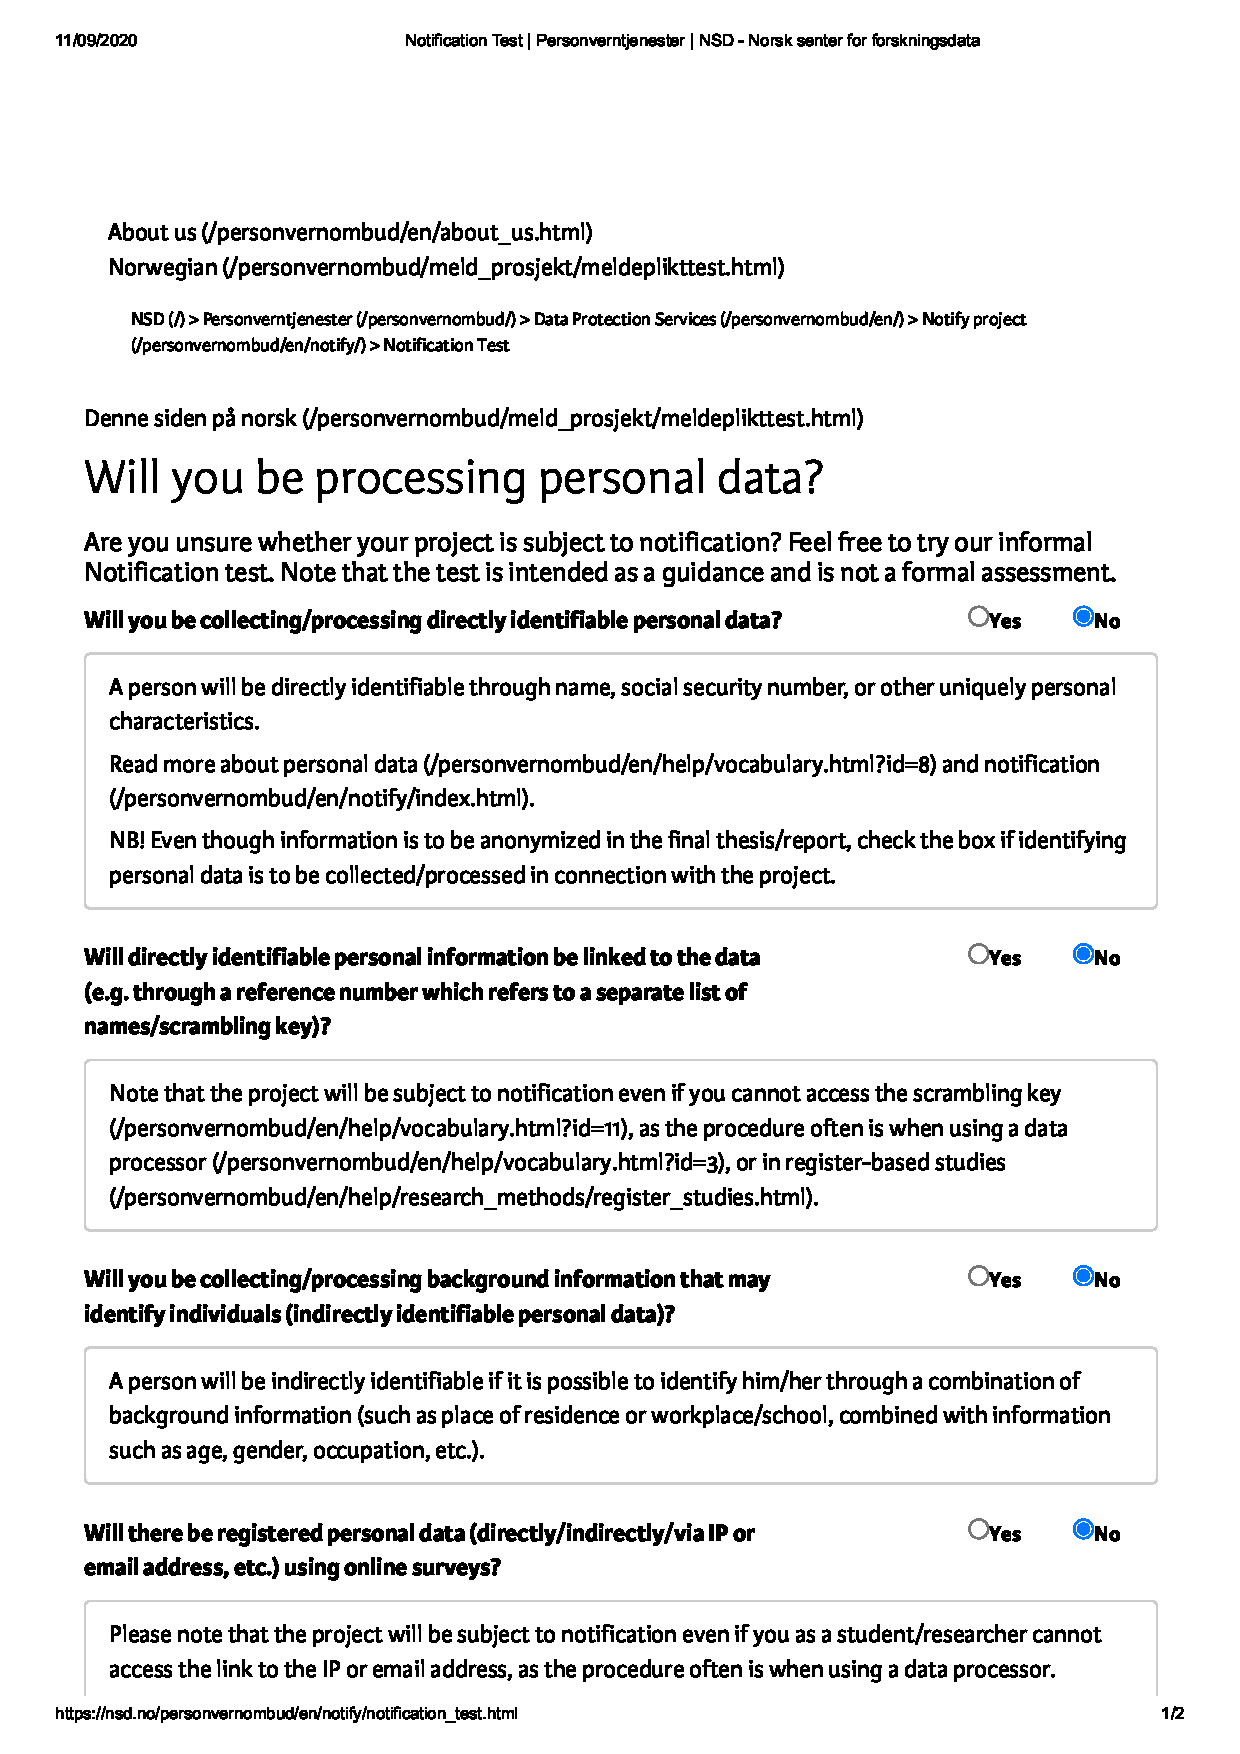
\includepdf[pages=-,fitpaper=true,noautoscale=true]{Notification-Test.pdf}
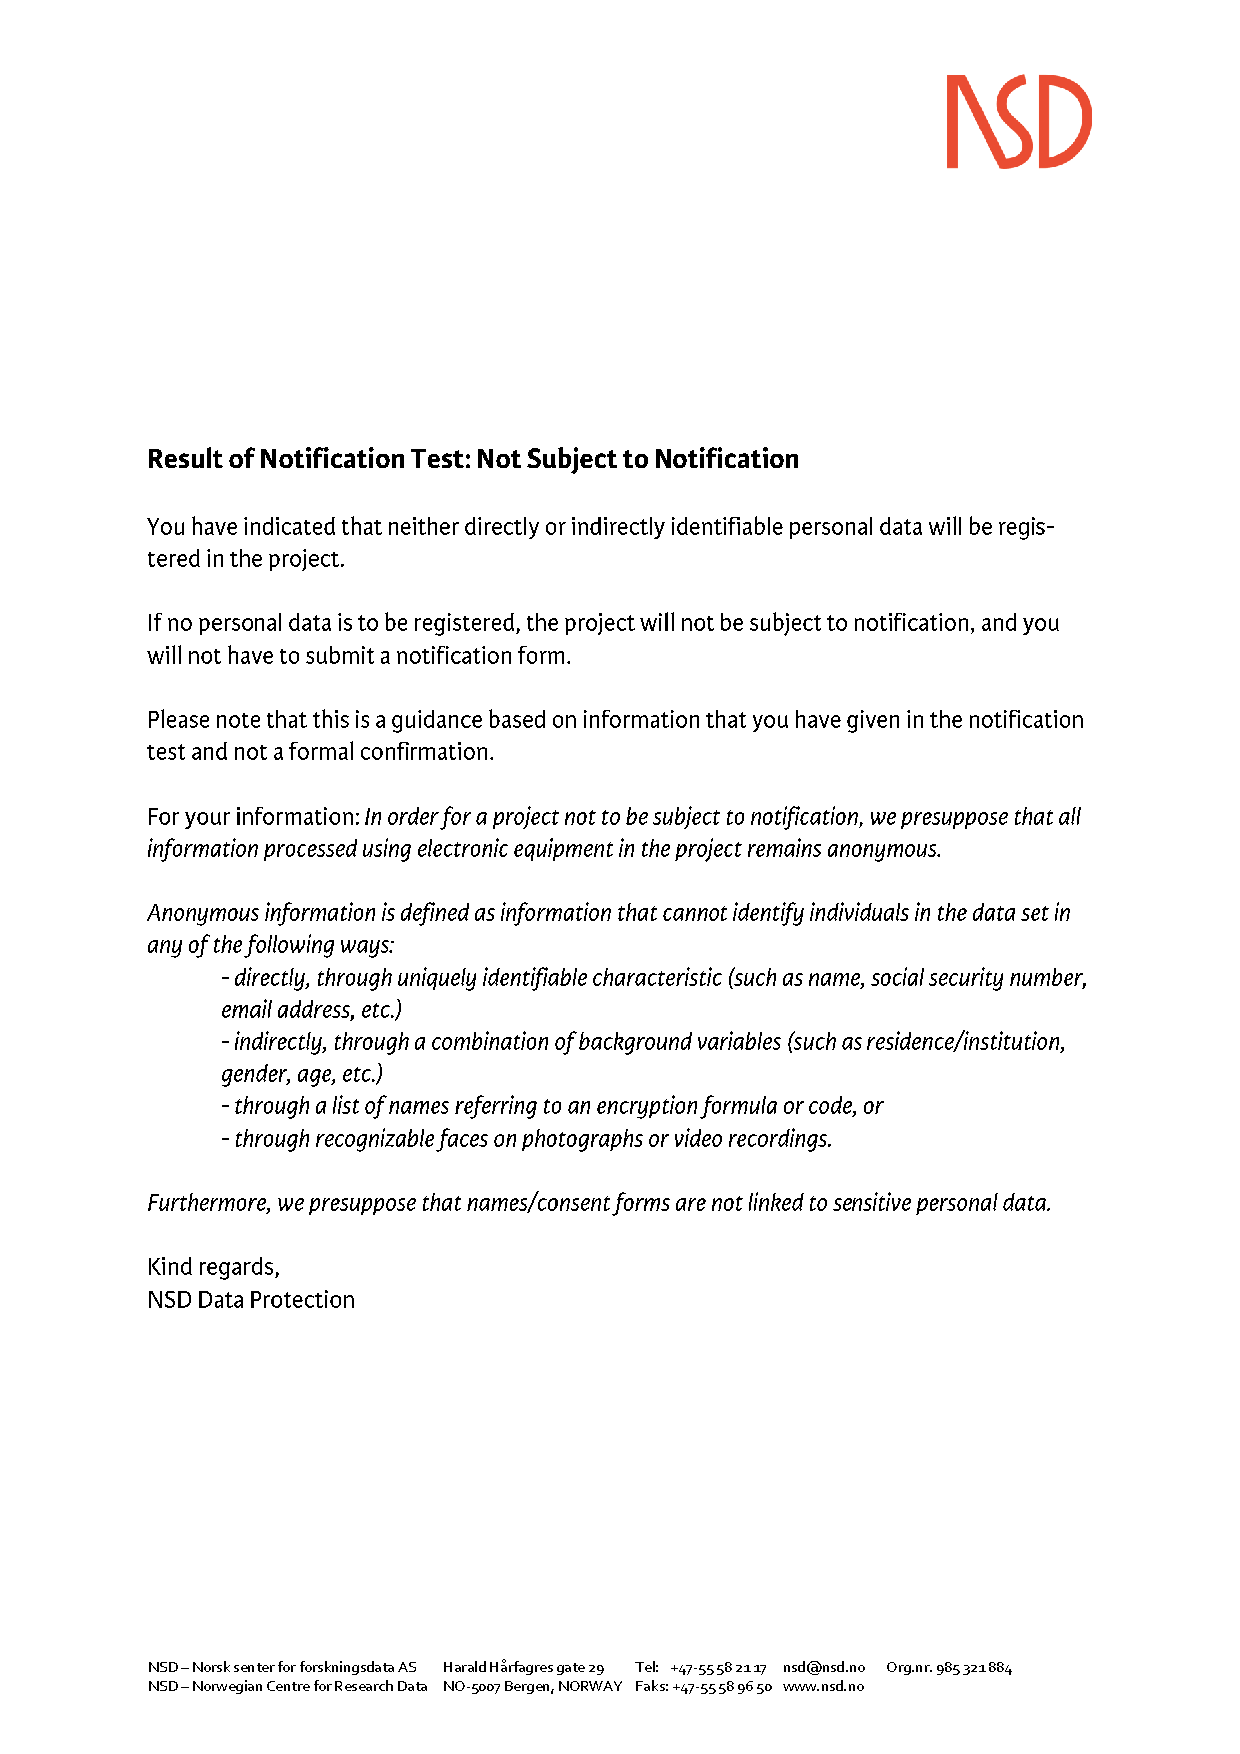
\includepdf[pages=-,fitpaper=true,noautoscale=true]{not_subject_to_notification.pdf}

\section{Data Management and Analysis Code}\label{app:B}

\appindent Data are publicly available and retrievable at \url{ThisWebpage} or indicate why they are not accessible. Short Sketch of concrete parts of the data you used if not clear from method section or for instance when pre/postprocessing applies and has been done by someone else (StatisticsNorway or company or ...).


R syntax for all data management steps and analyses related to this master thesis can be found at the following web page \url{GITHUB or OSF offer good platforms with free storage for this purpose}.

Do provide a quick overview of how you structured everything on those pages with pointers on what is what and can be found where. Keep it concise but  clear. The following parts can be found:
\begin{itemize}
    \item Data management: DATA.R
    \item Descriptives: DESC.R
    \item Analyses for RQ1: RQ1.R
    \item ...
\end{itemize}

\section{Supplemental material}\label{app:C}

\appindent Fusce interdum iaculis metus eu varius. Fusce nec nunc commodo massa pharetra imperdiet eget quis ipsum. Aliquam hendrerit porttitor congue. Quisque et malesuada nulla. Sed feugiat vel lectus sed hendrerit. Duis et eros eleifend, tempus mauris sed, euismod eros. Donec congue, dolor a finibus sodales, lectus nunc suscipit massa, at mollis massa libero non erat. Donec vel finibus est. Nunc sodales enim eget nunc posuere egestas. Nulla rhoncus commodo leo et dapibus.

\end{document}
